\section{ESP charges}

This sections describes how to calculate partial charges by fitting to the electro static potential (ESP). These charges are 
widely used in the context of force fields (\cite{Momany1978}, \cite{Cox1981}, \cite{Singh1984}, \cite{Besler1990}, CHELP: 
\cite{Chirlian1987}, CHELPG: \cite{Breneman1990}, RESP-charges: \cite{Bayly1993}, CHELP-BOW/CHELMO: \cite{Sigfridsson1998}, 
ESP-charge from multi-pole-moments: \cite{Hu2007}). FHI-aims implements a simple method for cluster calculation (molecules) as well as 
two methods for solids (periodic boundary conditions) \cite{Campana2009}, \cite{Chen2010}.\\
The starting point for these methods is the calculation of the electro static potential at a sufficiently high number of grid points 
outside the vdw radius of the atoms. To define a space region for the grid two parameters are necessary: a minimal radius and a
maximal radius around the atoms. These radii are defined as multiples of the vdw-radius of the atoms, see figure \ref{esp_radius} 
for details. The values for the vdw radii of most atoms in the periodic table have been taken from 
"http://de.wikipedia.org/wiki/Van-der-Waals-Radius" (\cite{Bondi1964}, \cite{Rowland1996}, \cite{Mantina2009}). For the generation 
of the points cubic grids are used. For cluster calculations points within a cube encapsulating the spheres with the maximal radius (multiple of the vdw radius) around all atoms are generated. For periodic boundary conditions the provided unitcell is used. The points within the superposition of the spheres with the minimal radius (minimal multiple of the vdw radius) are excluded.  The atom-centered radial grids are also available, mainly for test purposes. Here, all points lie on N spheres with radii between the minimal and maximal multiple of the vdw radius. The spacing between the radii of the N spheres is equidistant or logarithmic.\\
\begin{figure}[h]
\begin{center}
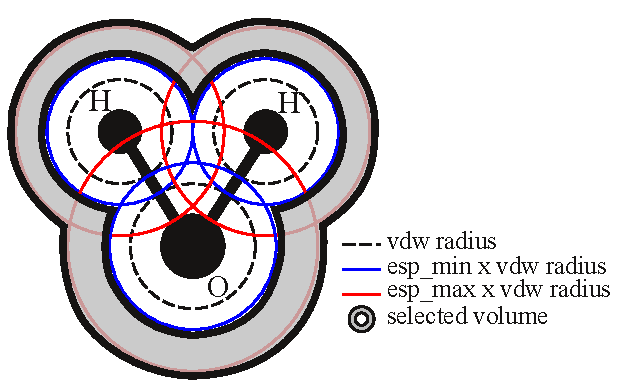
\includegraphics[height=9 cm]{esp_radius}
\end{center}
\caption{Definition of the volume used for the creation of grid points at which the potential is evaluated.} 
\label{esp_radius}
\end{figure}
For the cluster case the function to fit to is a sum of Coulomb potentials with charges $q_i$, the ESP-charges, 
at the atomic position $\mathbf{R}_i$:
\begin{equation}
 V_{ESP}(\mathbf{r})=\sum_{i=1}^{N_{at}}\frac{q_i}{|\mathbf{r}-\mathbf{R}_i|}
\end{equation}
The $q_i$ are calculated by a least squares fit with the additional constraint of constant total charge $q_{tot}=\sum_{i=1}^{N_{at}} q_i$. 
We use the method of Lagrange multipliers to minimize the function:
\begin{equation}
 F=\sum_{k=1}^{N_{grid}}\left(V_{DFT}(\mathbf{r_k})-V_{ESP}(\mathbf{r_k})\right)^2-\lambda\left(q_{tot}-\sum_{i=1}^{N_{at}}q_i\right)^2.\label{F_esp}
\end{equation}
This can be translated into a system of linear equations:
\begin{equation}
 \mathbf{\hat{A}}\mathbf{q}=\mathbf{B}.
\end{equation}
with the $N_{at+1}$ x $N_{at+1}$ matrix $\mathbf{\hat{A}}$:
\begin{align}
A_{ij}=&\sum_{k=1}^{N_{grid}}\frac{1}{|\mathbf{r_k}-\mathbf{R}_i|}\frac{1}{|\mathbf{r_k}-\mathbf{R}_j|}\quad \mathrm{with}\quad i,j\leq N_{at}\\
A_{i=N_{at}+1,j}=&A_{i,j=N_{at}+1}=1;\qquad A_{i=N_{at}+1,j=N_{at}+1}=0\nonumber
\end{align}
and the $N_{at}+1$ vector $\mathbf{B}$:
\begin{align}
 B_i=&\sum_{k=1}^{N_{grid}}\frac{V_{DFT}(\mathbf{r_k})}{|\mathbf{r_k}-\mathbf{R}_i|}\quad \mathrm{with}\quad i\leq N_{at}\\
 B_{i=N_{at}+1}=q_{tot}
\end{align}
$\mathbf{q}$ are the $N_{at}$ charges.\\
For solids (periodic boundary conditions) the situation is more complicated because all charges are repeated infinitely and the 
potential is only defined up-to an arbitrary offset. The methods to solve this problem are based on Ewald summation. 
Details on method 1 can be found here \cite{Campana2009} and on method two here \cite{Chen2010}. The function for the potential 
generated by the ESP charges centered at the atoms of the unit-cell now reads:
\begin{equation}
 V_{ESP}(\mathbf{r})=\sum_{i=1,\mathbf{T}}^{N_{at}}q_i\frac{\mathrm{erfc}(\alpha|\mathbf{r}-\mathbf{R_{i,\mathbf{T}}}|)}{|\mathbf{r}-\mathbf{R_{i,\mathbf{T}}}|}+\frac{4\pi}{V_{cell}}\sum_{i=1,\mathbf{k}}^{N_{at}}q_i\mathrm{cos}(\mathbf{k}(\mathbf{r}-\mathbf{R}_{i}))\frac{\mathrm{exp}^{-\frac{k^2}{4\alpha^2}}}{k^2}\label{V_Ewald}
\end{equation}
with $\mathbf{T}=n_1\mathbf{a}_1+n_2\mathbf{a}_2+n_3\mathbf{a}_3$ mapping the lattice positions. $\mathbf{a_i}$ the lattice vectors, 
$n_i \in \mathbb{Z}$. $\mathbf{k}=m_1\mathbf{b}_1+m_2\mathbf{b}_2+m_3\mathbf{b}_3$ mapping the reciprocal space. $\mathbf{b_i}$ the 
reciprocal lattice vectors, $m_i \in \mathbb{Z}$. $V_{cell}$ is the volume of the unit-cell. The parameter $\alpha$ is 
defined as $\alpha=\frac{\sqrt{\pi}}{R_c}$ with $R_c$ the cutoff radius of the 
Ewald summation. For the second method Wolf summation is implemented as well:
\begin{align}
 V_{ESP}(\mathbf{r})=&\sum_{i=1}^{N_{at}}q_i\left[\frac{\mathrm{erfc}(\sqrt{\alpha}|\mathbf{r}-\mathbf{R_{i}}|)}{|\mathbf{r}-\mathbf{R_{i}}|}-\frac{\mathrm{erfc}(\sqrt{\alpha}R_c)}{R_c}+\left(\frac{\mathrm{erfc}(\sqrt{\alpha}R_c)}{R_c^2}+\frac{2\sqrt{\alpha}}{\sqrt{\pi}}\frac{\mathrm{exp}(\alpha R_c^2)}{R_c}\right)\right]\label{V_Wolf}\\
                     &\mathrm{x}(|\mathbf{r}-\mathbf{R_{i}}|-R_c)\nonumber
\end{align}
The function to minimize for method 1 is:
\begin{align}
 F_1^{PBC}=&\sum_{k=1}^{N_{grid}}\left(V_{DFT}(\mathbf{r_k})-V_{ESP}(\mathbf{r_k})+\frac{1}{N_{grid}}\sum_{j=1}^{N_{grid}}\left(V_{DFT}(\mathbf{r_j})-V_{ESP}(\mathbf{r_j})\right)\right)^2\\\nonumber
           &-\lambda\left(q_{tot}-\sum_{i=1}^{N_{at}}q_i\right)+\sum_{i=1}^{N_{at}}w_i\left(E_i^0+\chi_i q_i+\frac{1}{2}J_i^{00}q_i^2\right). \label{F_esp_pbc1}
\end{align}
The $\chi_i$ and $J_i^{00}$ are electro-negativity and self-Coulomb interaction of the respective elements, which can be used to 
constrain the desired charges. $w_i$ are weighting factors for the constraints. This results in $\hat{A}$ and $\mathbf{B}$ for the 
linear equations system:
\begin{align}
 A_{ij}=\sum_{k=1}^{N_{grid}}&\left(\frac{\partial V_{ESP}(\mathbf{r_k})}{\partial q_i}-\frac{1}{N_{grid}}\sum_{j=1}^{N_{grid}}\frac{\partial V_{ESP}(\mathbf{r_j})}{\partial q_i}\right)~\mathrm{x}\\\nonumber
                             & \left(\frac{\partial V_{ESP}(\mathbf{r_k})}{\partial q_j}-\frac{1}{N_{grid}}\sum_{m=1}^{N_{grid}}\frac{\partial V_{ESP}(\mathbf{r_m})}{\partial q_j}\right)+\frac{w_i}{2}J_i^{00}\delta_{ij} \quad\mathrm{;}\quad i,j\leq N_{at}\\\nonumber
A_{i=N_{at}+1,j}=&A_{i,j=N_{at}+1}=1;\qquad A_{i=N_{at}+1,j=N_{at}+1}=0\\\nonumber
 B_{i}=\sum_{k=1}^{N_{grid}}&\left(V_{DFT}(\mathbf{r_k})-\frac{1}{N_{grid}}\sum_{j=1}^{N_{grid}}V_{DFT}(\mathbf{r_j})\right)~\mathrm{x}\\\nonumber
                             & \left(\frac{\partial V_{ESP}(\mathbf{r_k})}{\partial q_i}-\frac{1}{N_{grid}}\sum_{m=1}^{N_{grid}}\frac{\partial V_{ESP}(\mathbf{r_m})}{\partial q_i}\right)-w_m\frac{\chi_m}{2} \quad \mathrm{;} \quad i\leq N_{at}\\\nonumber
B_{i=N_{at}+1}&=q_{tot}\\\nonumber
\end{align}

The function to minimize for method 2 is:
\begin{align}
 F_2^{PBC}=&\sum_{k=1}^{N_{grid}}\left(V_{DFT}(\mathbf{r_k})-\left(V_{ESP}(\mathbf{r_k})+V_{DFT}^{offset}\right)\right)^2\\\nonumber
           &-\lambda\left(q_{tot}-\sum_{i=1}^{N_{at}}q_i\right)+\beta\sum_{i=1}^{N_{at}}\left(q_i-q_{i0}\right)^2. \label{F_esp_pbc2}
\end{align}
The constraint charges $q_{i0}$ can be determined with other methods (e.g. Mulliken charge analysis \cite{Mulliken55}), $\beta$ is the 
weighing factor. This gives $\hat{A}$ and $\mathbf{B}$:
\begin{align}
 &A_{ij}=\sum_{k=1}^{N_{grid}}\left(\frac{\partial V_{ESP}(\mathbf{r_k})}{\partial q_i}\frac{\partial V_{ESP}(\mathbf{r_k})}{\partial q_j}\right)+\beta\delta_{ij} \quad\mathrm{;}\quad i,j\leq N_{at}\\\nonumber
 &A_{i=N_{at}+1,j}=A_{i,j=N_{at}+1}=\sum_{k=1}^{N_{grid}}\frac{\partial V_{ESP}(\mathbf{r_k})}{\partial q_j}\quad j\leq N_{at}\\\nonumber
 &A_{i=N_{at}+2,j}=A_{i,j=N_{at}+2}=1\\\nonumber
 &A_{i=N_{at}+2,j=N_{at}+2}=A_{i=N_{at}+1,j=N_{at}+2}=A_{i=N_{at}+2,j=N_{at}+1}=0\\\nonumber
 &B_{i}=\sum_{k=1}^{N_{grid}}\left(V_{DFT}(\mathbf{r_k})\frac{\partial V_{ESP}(\mathbf{r_k})}{\partial q_i}\right)-\beta q_{0i} \quad \mathrm{;} \quad i\leq N_{at}\\\nonumber
 &B_{i=N_{at}+1}=\sum_{j=1}^{N_{grid}}V_{DFT}(\mathbf{r_j})\\\nonumber
 &B_{i=N_{at}+2}=q_{tot}\nonumber
\end{align}
Here the arbitrary offset of the potential $V_{offset}$ is an additional fitting parameter, the matrix $\hat{A}$ is of dimension $N_{at+2}$ x $N_{at+2}$ and $\mathbf{B}$  of dimension $N_{at+2}$. 
For method 1 $V_{offset}$ can be calculated as:
\begin{equation}
 V_{offset}=\sum_{k=1}^{N_{grid}}\left( V_{DFT} (\mathbf{r_k})-V_{ESP}(\mathbf{r_k})\right)
\end{equation}
from the fitted charges $q_i$. As a measure for the quality of the fit the root-mean-square ($RRMS$) is defined as:
\begin{equation}
 RRMS=\left\{\frac{\sum_{k=1}^{N_{grid}}\left(\left(V_{ESP}(\mathbf{r_k})+V_{offset}\right)-V_{DFT}(\mathbf{r_k})\right)^2}{\sum_{k=1}^{N_{grid}}\left(V_{DFT}(\mathbf{r_k})\right)^2}\right\}^2
\end{equation}
The current implementation is quite sensitive to the points chosen for the calculation of the electrostatic potential. Thorough studies 
regarding the parameters for the grid are advised! For periodic boundary conditions the ESP-charges calculated for transition densities 
are experimental, caution!! The ESP-charges from transition densities can be benchmarked against the dipole-moments calculated with 
\keyword{compute\_dipolematrix}.\\
Example for a periodic system: 
\begin{verbatim}
      output esp
      esp n_radius 10
      esp radius 1.0 2.
      esp pbc_method 1
      esp R_c 10
      output esp
      esp n_radius 10
      esp radius 1.0 2.
      esp pbc_method 2
      esp R_c 30
      output esp
      esp radius 1.0 2.
      esp pbc_method 2
      esp R_c 20
      esp equal_grid_n 10 10 10
\end{verbatim}
The ESP-charges for the full potential will be calculated for a periodic system. At first with points within once the vdw radius 
and twice the vdw radius of the atoms, with 10 shells in between and a cutoff radius of 10$\AA$ for the Ewald summation, method 1 
(Ewald summation) is used. Secondly with points within once the vdw radius and twice the vdw radius of the atoms, with 10 shells in 
between and a cutoff radius of 30$\AA$, method 2 (Ewald summation) is used. Thirdly with points within once the vdw radius and twice 
the vdw radius of the atoms, with 10$\times$10$\times$10 initial points on a cubic grid, method 2 is used.\\

\textbf{Warning}: For periodic boundary conditions the atoms in the supplied \texttt{geometry.in} must be within the first (central) Wigner-Seitz-cell. 
For a two layer system it would normally be possible to have one layer within the (central) Wigner-Seitz-cell and the second one sticking out at 
one side. Periodic boundary conditions will take care. The atoms sticking out would be shifted back into the (central) Wigner-Seitz-cell. 
This might lead to different ESP-charges and Dipole matrix elements. They are only invariant for collective translations of all atoms. 
The program will stop if a non-valid geometry is detected.
\newpage


\subsection*{Tags for general section of \texttt{control.in}:}
\subkeydefinition{output}{esp}{control.in}
{
  \noindent
  Usage: \keyword{output} \subkeyword{output}{esp}\\[1.0ex]
  Purpose: Calculate the ESP-charges at the atomic position from the full density with default settings. The default settings are to 
  use a radial grid with equidistant radii and without mapping back to the unit-cell in case of periodic boundary conditions. The radial 
  multipliers for the exclusion radius are 3 (Minimum) and 8 (Maximum) times the vdw-radius for the cluster case and 
  1 (Minimum) and 2 (Maximum) times the vdw-radius for pbc. In both cases 5 radial-shells are used. For pbc a cutoff radius for 
  the Ewald summation of 10$\mathrm{\AA}$ is used. The maximal multiples of the lattice vectors ($r_m$) and the reciprocal 
  lattice vectors ($k_m$) used in the summation are 7 (for both). No constraints are applied to the charges.\\
  The keyword can be used multiple times to calculate esp charges with different settings. The optional sub-sub keywords 
  (see below) have to be set after \keyword{output} \subkeyword{output}{esp} for every calculation separately, 
   otherwise defaults are used.\\}
Optional keywords for \keyword{output} \subkeyword{output}{esp}:\\
\begin{itemize}
\item \subkeyword{output}{esp} \texttt{spin} \textit{spin} \\
  Select \textit{spin} spin state (1 or 2) for the calculation of the esp charges from the transition density $\rho_{ij}$ with 
  states i -> j (default 1) at k-point \textit{kpoint} (default 1).
\item \subkeyword{output}{esp} \texttt{state} \textit{state\_one state\_two} \\
  Select states i=\textit{state\_one} -> j=\textit{state\_two} (i,j $\in$ [1,n\_states]) for the calculation of the esp charges 
  from the transition density $\rho_{ij}$ with spin \textit{spin} (default 1) at k-point \textit{kpoint} (default 1).
\item \subkeyword{output}{esp} \texttt{kpoint} \textit{k-point} \\
  Select states the \texttt{kpoint} (\textit{k-point} $\in$ [1,n\_k\_points]) for the calculation of the esp charges 
  from the transition density $\rho_{ij}$ states i -> j (default 1) with spin \textit{spin} (default 1).
\item \subkeyword{output}{esp} \texttt{radius} \textit{min\_radius max\_radius} \\
  Select the minimal (min\_radius) and maximal (max\_radius) multiple of the vdw radius to select the volume where the 
  potential is evaluated and the esp charges fitted. Defaults: 3 and 8 for clusters and 1 and 2 for pbc. \textit{max\_radius} should not 
  be larger than smallest lattice vector for pbc and radial gird.
\item \subkeyword{output}{esp} \texttt{n\_radius} \textit{n\_radius} \\
  Select the \textit{n\_radius} number of of radial shells that are used to create points in the selected volume. Default: 5
\item \subkeyword{output}{esp} \texttt{equal\_grid\_n} \textit{n\_grid\_x} \textit{n\_grid\_y} \textit{n\_grid\_z}\\
  Select the number of points for the cubic grid in x - \textit{n\_grid\_x}, y -  \textit{n\_grid\_y} and z - \textit{n\_grid\_z} direction. Default: 10 10 10
\item \subkeyword{output}{esp} \texttt{rm} \textit{r\_m} \\
  PBC only. Maximum number \textit{r\_m} of multiples of the lattice vectors that are used in the real space sum of the Ewald summation. 
  Default: 7
\item \subkeyword{output}{esp} \texttt{km} \textit{k\_m} \\
  PBC only. Maximum number \textit{k\_m} of multiples of the reciprocal lattice vectors that are used in the reciprocal space sum of the Ewald summation. 
  Default: 7
\item \subkeyword{output}{esp} \texttt{R\_c} \textit{R\_c} \\
  PBC only. Real space cutoff radius for the Ewald/Wolf-summation. Default: 20$\mathrm{\AA}$.
\item \subkeyword{output}{esp} \texttt{pbc\_method} \textit{method} \\
  PBC only. Switch between methods for periodic boundary conditions. Choices for \textit{method}: \textit{1} - method 1 
  with Ewald summation (\ref{F_esp_pbc1}, \ref{V_Ewald}); \textit{2} - method 2 with Ewald summation (\ref{F_esp_pbc2}, 
  \ref{V_Ewald});   \textit{3} - method 3 with Wolf summation (\ref{F_esp_pbc2}, \ref{V_Wolf}). Default: 2
\item \subkeyword{output}{esp} \texttt{grid} \textit{type}\\
  Switch between radial gird - 1, logarithmic radial grid - 2, cubic grid from lattice vectors - 3 and cubic grid from lattice vectors, but truncated in z-direction by maximal vdw-radius (exclude vacuum region for surface slabs) - 4. Default: 3. 
\item \subkeyword{output}{esp} \texttt{output\_cube} \textit{type}\\
  Instead of fitting the ESP-charges to the potential, the potential is written to a cube-file (potential\_esp\_i.cube).  A cubic grid is required. Switch between Hartree potential - 1, XC-potential - 2,  X-potential - 3, C-potential - 4, Density - 5, and Hartree potential with the coordinates of voxels - 6.
\item \subkeyword{output}{esp} \texttt{output\_fit}\\
  The ESP-charges are fitted to the potential and the potential calculated from the fitted ESP-charges is written to a cube-file (potential\_esp\_i.cube). A cubic grid is required.
\item \subkeyword{output}{esp} \texttt{use\_dip\_for\_cube}\\
  The dipole correction is added to the cube output of the (fitted) potential. Only applied if a dipole correction was used during SCF. 

  \end{itemize}
\keydefinition{esp\_constraint}{control.in}
{
  \noindent
  Usage: \keyword{esp\_constraint} \option{method}\\[1.0ex]
  Purpose: PBC only. Constrain the calculated ESP charges with periodic boundary conditions for method 1 or 2. The constraints 
  will be used for all calculated ESP-charges. Due to technical reasons (array allocations) you have to specify the method 
  you are using in \textit{control.in} with this keyword. Choices for \option{method} are \textit{1} and \textit{2}. The actual 
  constraints have to be specified for each atom in \textit{geometry.in}.\\[1.0ex]
}
\keydefinition{compute\_esp\_charges}{control.in}
{
  \noindent
  Usage: \keyword{compute\_esp\_charges} \option{$E_{min}$} \option{$E_{max}$} \option{min\_vdw\_radius} \option{grid\_type} \option{max\_vdw\_radius} \option{n\_radius} \option{k-point}\\[1.0ex]
  Purpose: Calculate and output the  ESP-charges for the transition states within the energy window [\option{$E_{min}$}, \option{$E_{max}$}] at 
  k-point \option{k-point}. Data will be written to file \textit{esp\_element\_}\option{k-point}\textit{.dat}.
  The grid type \option{grid\_type} (1 - radial, 2 - logarithmic radial, 3 - cubic, 4 - cubic from radii) will be used. The potential 
  will be calculated on the \option{n\_radius} radial shells within the volume created by \option{min\_vdw\_radius} and \option{max\_vdw\_radius} 
  times the vdw radius of the atoms or in a cube with \option{n\_radius}x\option{n\_radius}x\option{n\_radius} oints. The dipole moment calculated from the fitted charges $q_i$ at atomic positions $R_i$ is 
  also written to file:
  \begin{equation}
   \mathbf{d_{ij}}=\sum_{k=1}^{N_{at}}q_k\mathbf{R_k}
  \end{equation}
  for transition states $ i \rightarrow j$.\\[1.0ex]
}
\subsection*{Tags for \texttt{geometry.in}:}
\keydefinition{esp\_constraint}{geometry.in}
{
  \noindent
  Usage: \keyword{esp\_constraint} \option{constraint\_1} \option{constraint\_2} \option{constraint\_3}\\[1.0ex]
  Purpose: PBC only. Define the constraints for the fit of the ESP-charges for each atom. Depending on the chosen method 
  (\keyword{esp\_constraint} \option{method} in \textit{control.in}). Method 1 needs three parameters ($\chi, J^{00}, w$) \ref{F_esp_pbc1}
  and method 2 needs two parameters ($q_0, \beta$) \ref{F_esp_pbc2} as defined above.\\[1.0ex]
}
